\onehalfspacing
\fancypagestyle{plain}{
	\fancyhf{}
	\rhead{\thepage}
	\renewcommand{\headrulewidth}{0pt}
	\renewcommand{\footrulewidth}{0pt}
}

\chapter{DISEÑO Y DESARROLLO DEL PROYECTO}

\section{Esquematización y arquitectura del sistema}

\subsection{Diseño mecánico del concepto óptimo}

\begin{figure}[H]
	% Fuerza la alineación izquierda y quita los ":" después del número
	\captionsetup{justification=raggedright, singlelinecheck=false, labelsep=none}
	
	\caption[Vista general del concepto óptimo.]{} 
	
	% Vspace negativo opcional para acercar el texto cursivo al número de figura
	\textit{Vista general del concepto óptimo.} \par\medskip
	
	\centering
	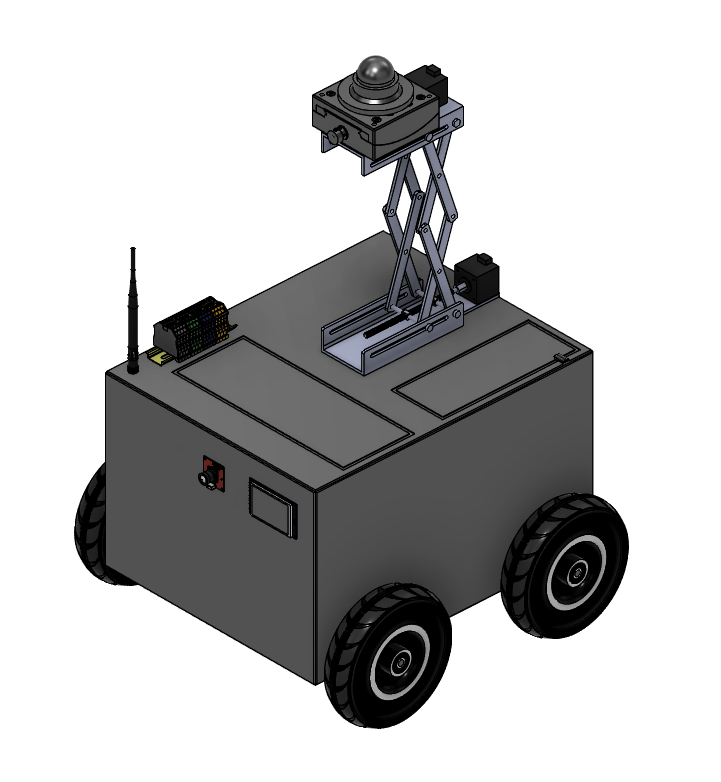
\includegraphics[width=0.6\textwidth]{Recursos/Imagenes/ImagenesSolucionOptima/CAD-GENERAL_V1.png} \par\medskip
	
	\raggedright
	\footnotesize \textit{Nota.} Elaboración propia.
	\label{fig:CADGENERAL}
\end{figure}

\subsubsection{Subsistema de traslación}

El subsistema de traslación está representado en la Figura \ref{fig:SubsistemaTraslacion}. El movimiento principal del mecanismo permite el avance longitudinal y el giro mediante tracción diferencial.

\begin{figure}[H]
	\captionsetup{justification=raggedright, singlelinecheck=false, labelsep=none}
	\caption[Vista isométrica y frontal del subsistema de traslación.]{} 
	\textit{Vista isométrica y frontal del subsistema de traslación.} \par\medskip
	
	\begin{minipage}{0.5\textwidth}
		\centering
		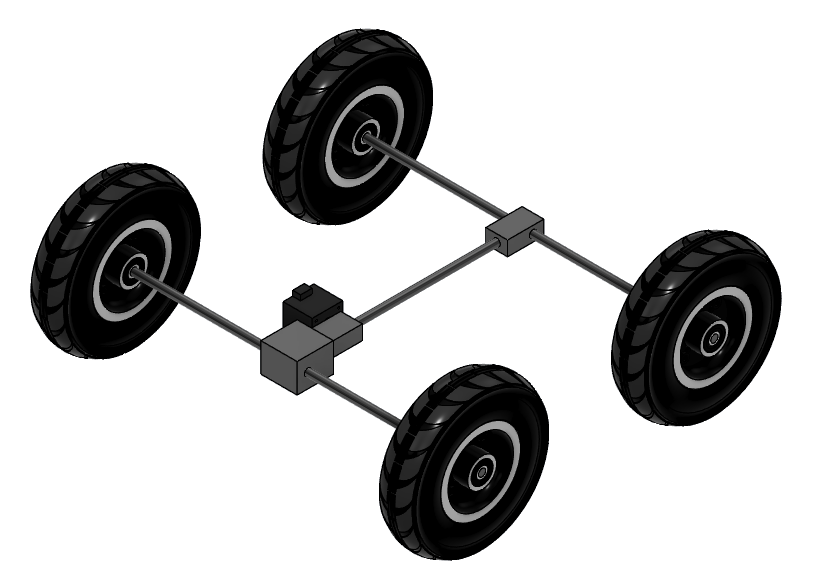
\includegraphics[width=\linewidth]{Recursos/Imagenes/ImagenesSolucionOptima/SISTEMA_TRASLACION_ISO.png}
	\end{minipage}\hfill
	\begin{minipage}{0.5\textwidth}
		\centering
		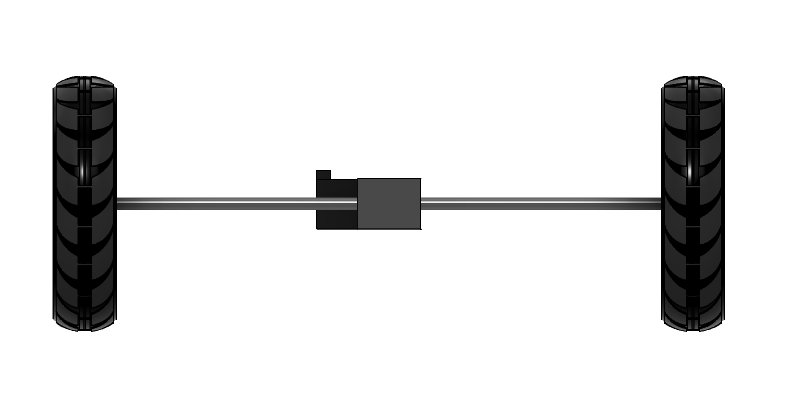
\includegraphics[width=\linewidth]{Recursos/Imagenes/ImagenesSolucionOptima/SISTEMA_TRASLACION_FRONT.png}
	\end{minipage}
	\par\medskip
	
	\raggedright
	\footnotesize \textit{Nota.} Las flechas rojas indican los grados de libertad y dirección del accionamiento mecánico para el desplazamiento. Elaboración propia.
	\label{fig:SubsistemaTraslacion}
\end{figure}

\subsubsection{Subsistema de posicionamiento de plataforma de medición}

En la Figura \ref{fig:SubsistemaPosicionamiento} se detalla el subsistema de posicionamiento, mecanismo de elevación por tijera accionado por un servomotor. Su función es ejecutar el movimiento rectilíneo de posicionamiento vertical para elevar la instrumentación. Gracias a su propiedad de autobloqueo, el servomotor retiene la altura frente a las vibraciones del terreno.

\begin{figure}[H]
	\captionsetup{justification=raggedright, singlelinecheck=false, labelsep=none}
	\caption[Vista isométrica y derecha del subsistema de posicionamiento.]{} 
	\textit{Vista isométrica y derecha del subsistema de posicionamiento.} \par\medskip
	
	\begin{minipage}{0.5\textwidth}
		\centering
		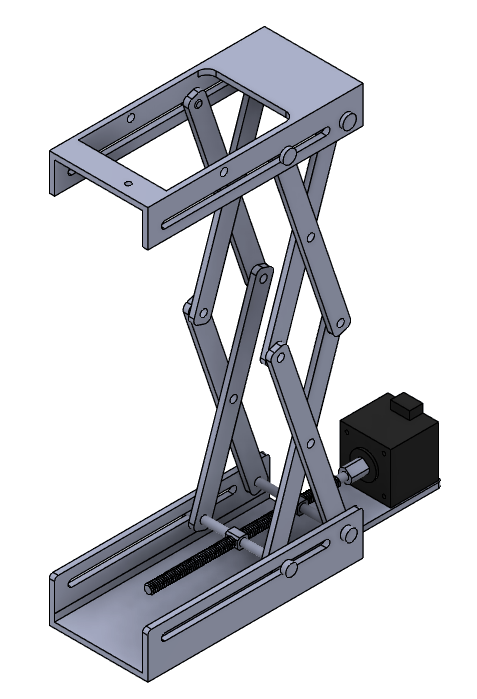
\includegraphics[width=\linewidth]{Recursos/Imagenes/ImagenesSolucionOptima/MECANISMO_POSICION_ISO.png}
	\end{minipage}\hfill
	\begin{minipage}{0.5\textwidth}
		\centering
		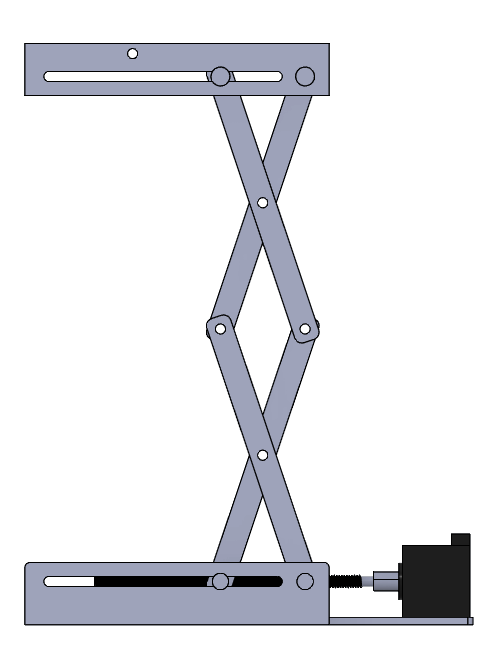
\includegraphics[width=\linewidth]{Recursos/Imagenes/ImagenesSolucionOptima/MECANISMO_POSICION_DERECHA.png}
	\end{minipage}
	\par\medskip
	
	\raggedright
	\footnotesize \textit{Nota.} Las flechas rojas indican la dirección del desplazamiento lineal vertical. Elaboración propia.
	\label{fig:SubsistemaPosicionamiento}
\end{figure}

\subsubsection{Subsistema de orientación de plataforma de medición}

El subsistema de orientación, como se observa en la Figura \ref{fig:SubsistemaOrientacion}, es el encargado de ejecutar el movimiento rotacional de ajuste (cabeceo o \textit{pitch}) de la plataforma superior. Este grado de libertad permite alinear estrictamente los piranómetros según las exigencias de horizontalidad de la norma IEC 61724-1, manteniendo la posición inalterable ante las ráfagas de viento gracias al mecanismo de retención interno.

\begin{figure}[H]
	\captionsetup{justification=raggedright, singlelinecheck=false, labelsep=none}
	\caption[Vista isométrica y derecha del subsistema de orientación.]{} 
	\textit{Vista isométrica y derecha del subsistema de orientación.} \par\medskip
	
	\begin{minipage}{0.5\textwidth}
		\centering
		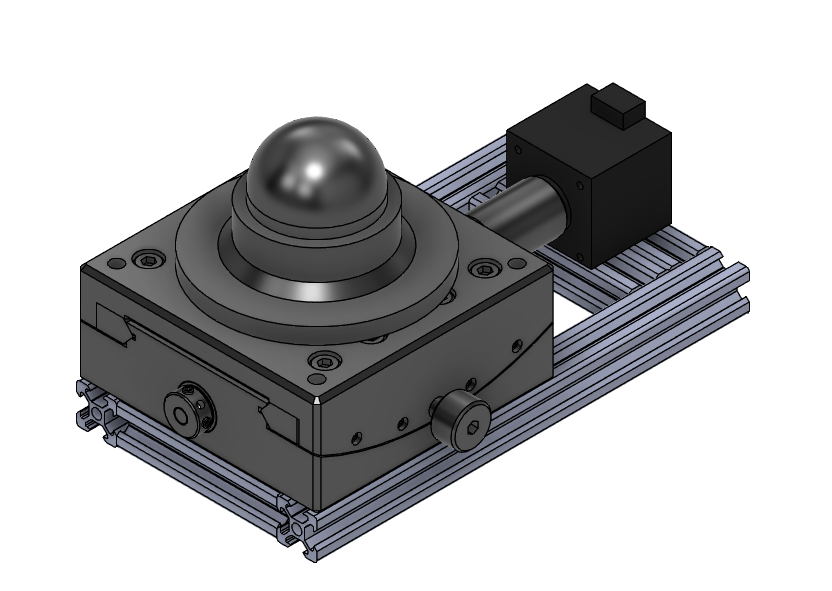
\includegraphics[width=\linewidth]{Recursos/Imagenes/ImagenesSolucionOptima/MECANISMO-ORIENTACION-ISO.png}
	\end{minipage}\hfill
	\begin{minipage}{0.5\textwidth}
		\centering
		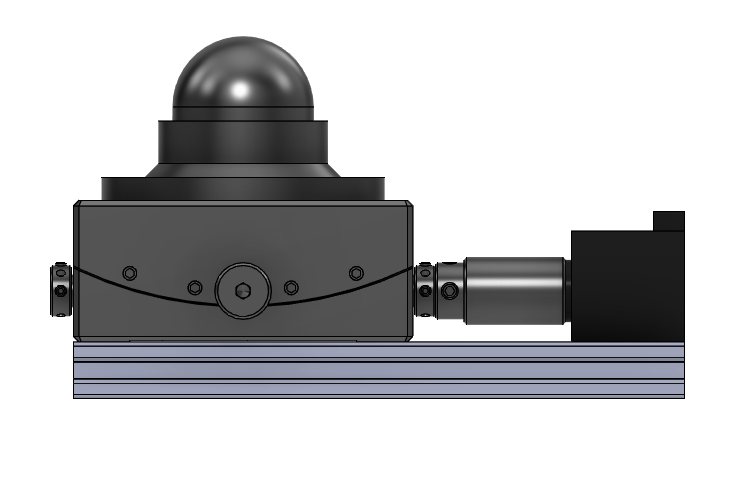
\includegraphics[width=\linewidth]{Recursos/Imagenes/ImagenesSolucionOptima/MECANISMO-ORIENTACION-DERECHA.png}
	\end{minipage}
	\par\medskip
	
	\raggedright
	\footnotesize \textit{Nota.} Las flechas rojas detallan el eje de rotación para la orientación de la instrumentación. Elaboración propia.
	\label{fig:SubsistemaOrientacion}
\end{figure}

\subsubsection{Estructura de soporte}

Finalmente, en la Figura \ref{fig:CarcasaISO} se presenta la estructura de soporte principal, conformada por un chasis de aluminio. Esta carcasa actúa como un escudo físico estático que aísla de forma hermética los componentes electrónicos de control y las baterías contra el ingreso de suciedad y las perturbaciones propias del entorno.

\begin{figure}[H]
	\captionsetup{justification=raggedright, singlelinecheck=false, labelsep=none}
	\caption[Vista isométrica de la estructura.]{} 
	\textit{Vista isométrica de la estructura.} \par\medskip
	
	\centering
	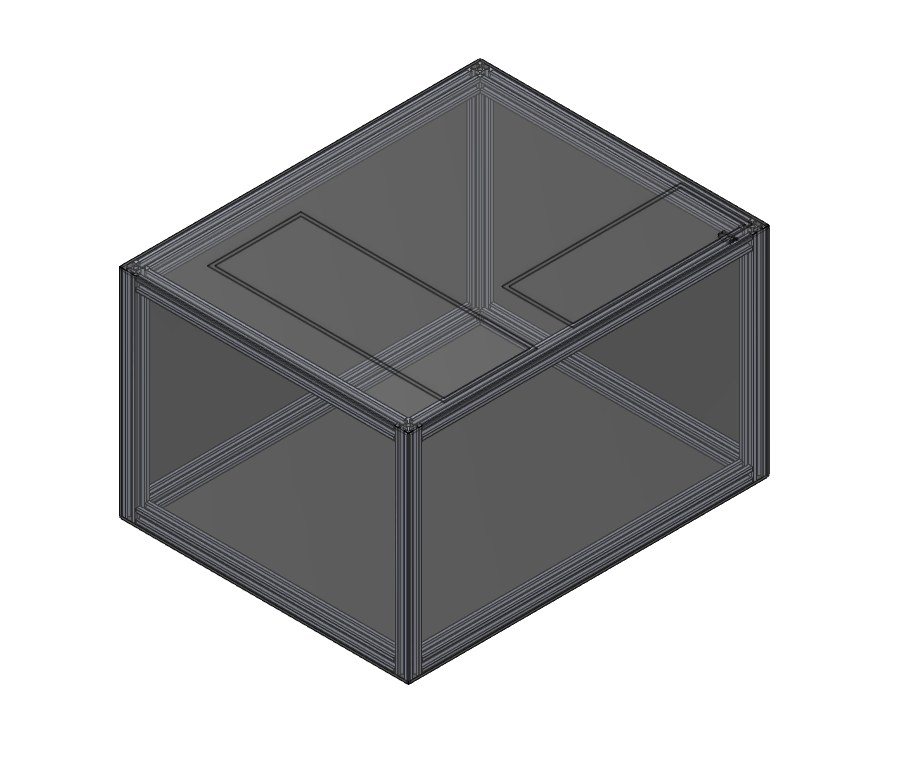
\includegraphics[width=0.8\textwidth]{Recursos/Imagenes/ImagenesSolucionOptima/SOPORTE-CUBIERTA-ISO.png} \par\medskip
	
	\raggedright
	\footnotesize \textit{Nota.} Elaboración propia.
	\label{fig:CarcasaISO}
\end{figure}


\subsection{Diseño integrador}
\subsubsection{Diagrama de operaciones}

Para diferenciar las responsabilidades y los canales de interacción de cada actor identificado en el análisis de stakeholders, la descripción se divide en dos diagramas independientes: el Usuario Principal (Técnico de O\&M en campo) y el Usuario Directo (Gestor de Activos y Auditor O\&M remoto).En ambos esquemas, se utiliza la simbología estandarizada donde los símbolos circulares representan procedimientos o comandos ejecutados por el usuario, mientras que los rombos y rectángulos representan subrutinas, decisiones lógicas y respuestas automáticas ejecutadas por el robot.

El flujo de trabajo en campo consta de cuatro fases secuenciales y paralelas:

El procedimiento inicia en el taller o punto de alistamiento de la planta fotovoltaica. El técnico realiza la inspección óptica del domo del piranómetro Clase A y de la lente del módulo de cámara CMOS. A continuación, inserta en la ranura externa la tarjeta de memoria MicroSD con el archivo de coordenadas de los pasillos, y acciona el interruptor principal. La SBC arranca el sistema operativo, ejecuta el autodiagnóstico de buses y despliega la lectura de estado en la pantalla LCD local. A continuación, el técnico traslada el UGV a la cabecera del pasillo entre seguidores solares, selecciona la ruta navegando en la pantalla LCD local y presiona el botón de confirmación en la interfaz LCD para autorizar el inicio del ciclo autónomo. En la siguiente fase, la SBC ejecuta tres hilos concurrentes en tiempo real:
\begin{itemize}
    \item \textbf{Inspección Climática:} El servomotor del elevador de tijera despliega la plataforma a una altura $h \ge 1300 \text{ mm}$ del suelo, mientras el goniómetro de 1 eje  alinea el piranómetro Clase A con el ángulo Tilt de los paneles. La tracción diferencial avanza siguiendo el algoritmo Pure Pursuit.
    \item \textbf{Percepción y Evasión Local:} La cámara CMOS frontal monitorea un semicírculo de $1 \text{ m}$. Si se detecta un obstáculo (maleza, rocas o herramientas), la SBC calcula una desviación local, esquiva el obstáculo, se reincorpora al pasillo fotovoltaico y continúa la misión de medición sin interrumpir el recorrido.
    \item \textbf{Supervisión Energética:} El contador de Culombios del BMS monitorea la descarga de las celdas. Únicamente si el nivel cae por debajo del $15\%$, el sistema aborta la inspección, repliega los mecanismos articulados a posición de transporte y ejecuta la subrutina de Retorno Automático navegando de vuelta al punto inicial del pasillo.
\end{itemize}

Finalmente, al llegar a la cabecera inicial (por ruta completada o retorno por batería baja), el robot notifica el mensaje en la pantalla LCD local. El técnico apaga el equipo desde el seccionador, extrae la tarjeta MicroSD para el respaldo no volátil de la base de datos climática, limpia el piranómetro y conecta la batería al cargador comercial.

El siguiente flujo describe la operación del auditor o gestor de telemetría, el cual accede al Dashboard web del centro de control mediante credenciales encriptadas. La plataforma establece comunicación inalámbrica con el Gateway central del parque solar, verificando los indicadores de calidad de radiofrecuencia y desplegando la cartografía vectorial de los pasillos; a continuación, el usuario configura la frecuencia de transmisión telemétrica y emite la instrucción inalámbrica de inicio, el paquete se transmite por LoRa al robot.Durante el desplazamiento del UGV en el pasillo, el servidor decodifica continuamente las tramas de carga útil enviadas por el robot. Si se detecta una condición crítica, el Dashboard resalta la alerta en color rojo en el mapa GPS exacto, permitiendo al gestor pulsar el botón de Parada Remota de Emergencia vía LoRa. Al concluir el recorrido, el robot emite la trama de cierre de ruta. El auditor ejecuta el algoritmo de integración climática para calcular el PR definitivo de la planta corregido por temperatura, cuantifica las pérdidas asociadas al soiling y exporta el informe técnico-económico de auditoría en formato PDF/Excel para sustentar las garantías de generación ante los inversionistas u operadores de red.

\begin{figure}[H]
	\captionsetup{justification=raggedright, singlelinecheck=false, labelsep=none}
	\caption[Flujo de operación del Usuario Principal.]{} 
	\textit{Flujo de operación del Usuario Principal.} \par\medskip
	
	\centering
	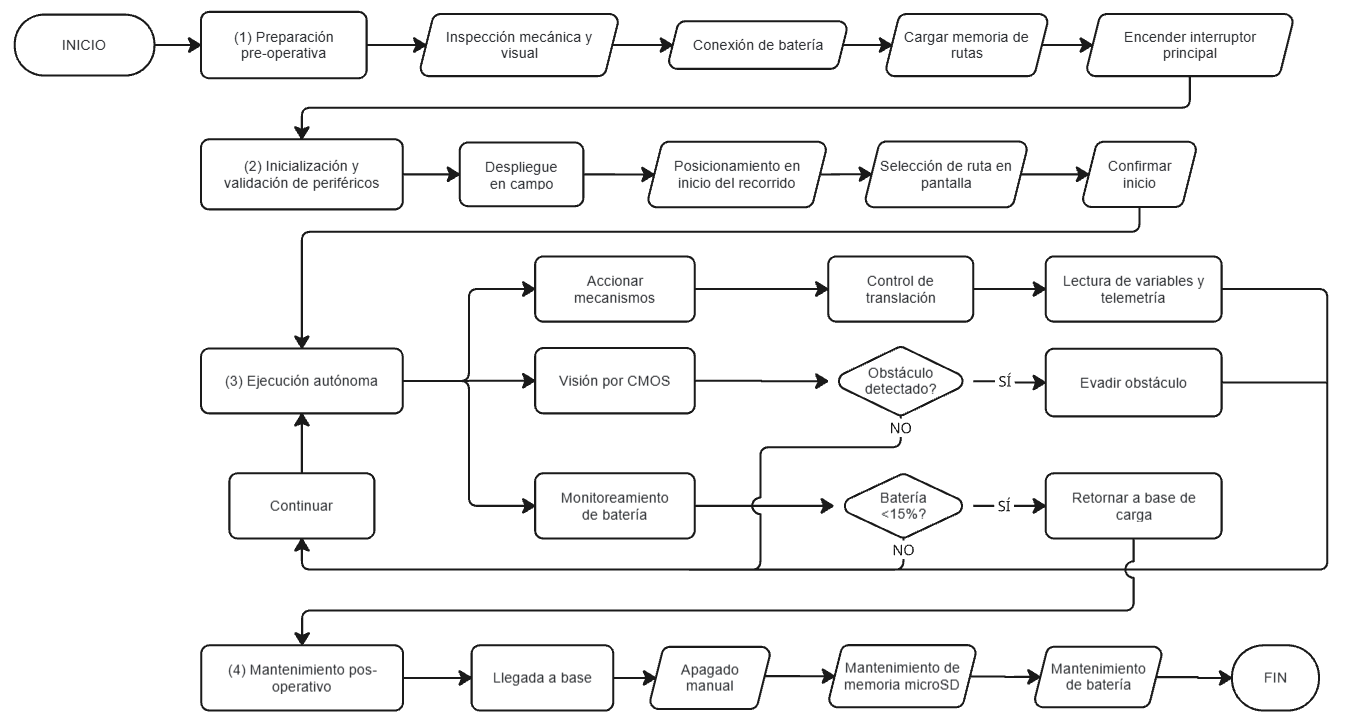
\includegraphics[width=0.8\textwidth]{Recursos/Imagenes/ImagenesDisenoOptimo/FlujoOperaciones1.png} \par\medskip
	
	\raggedright
	\footnotesize \textit{Nota.} Elaboración propia.
	\label{fig:DiagramaOperaciones1}
\end{figure}

\begin{figure}[H]
	\captionsetup{justification=raggedright, singlelinecheck=false, labelsep=none}
	\caption[Flujo de operación de.]{}
	\textit{Flujo de operación de.} \par\medskip
	
	\centering
	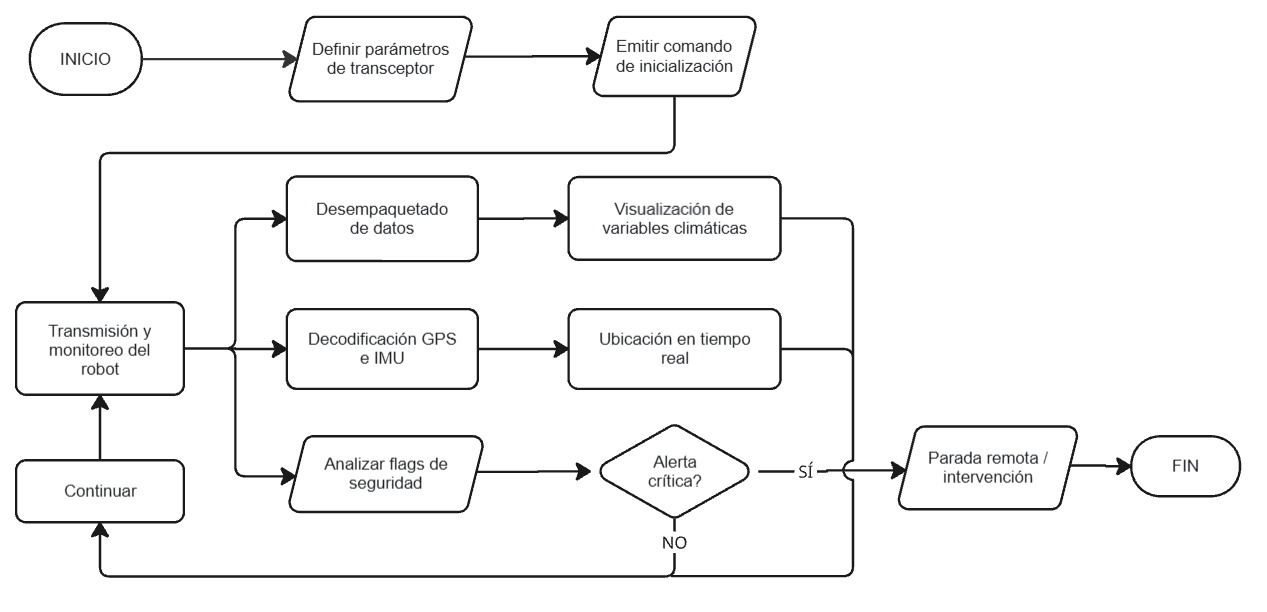
\includegraphics[width=0.8\textwidth]{Recursos/Imagenes/ImagenesDisenoOptimo/FlujoOperaciones2.png} \par\medskip
	
	\raggedright
	\footnotesize \textit{Nota.} Elaboración propia.
	\label{fig:DiagramaOperaciones2}
\end{figure}


\subsubsection{Diagrama de bloques} 

La Figura \ref{fig:DiagramaBloques}, ilustra la integración de hardware del concepto de solución seleccionado, segmentada según las interfaces de potencia y datos. La matriz energética está constituida por un paquete de baterías Li-Ion gestionado por un sistema BMS, el cual fluye a través de fusibles electrónicos que otorgan protección activa contra cortocircuitos. Desde este punto, la energía se bifurca hacia convertidores Buck DC-DC y reguladores lineales que independizan y estabilizan los niveles de tensión para aislar el ruido eléctrico entre la electrónica de control y la carga inductiva de los actuadores.

En el nivel de procesamiento, la Placa SBC actúa como el nodo maestro. A través de sus buses de datos digitales, consolida la conexión con los dispositivos periféricos: la antena GPS, la unidad IMU, la memoria MicroSD y el módulo de comunicaciones LoRa. Paralelamente, adquiere las lecturas analógico-digitales de la cámara CMOS frontal y los sensores meteorológicos. Finalmente, los pines de salida del microprocesador comandan los drivers de potencia que accionan los motores de tracción DC y los servomotores responsables de la cinemática de la plataforma de instrumentación.

\begin{figure}[H]
	\captionsetup{justification=raggedright, singlelinecheck=false, labelsep=none}
	
	\caption[Diagrama de bloques representativo de la arquitectura eléctrica.]{} 
	
	\textit{Diagrama de bloques representativo de la arquitectura eléctrica.} \par\medskip
	
	\centering
	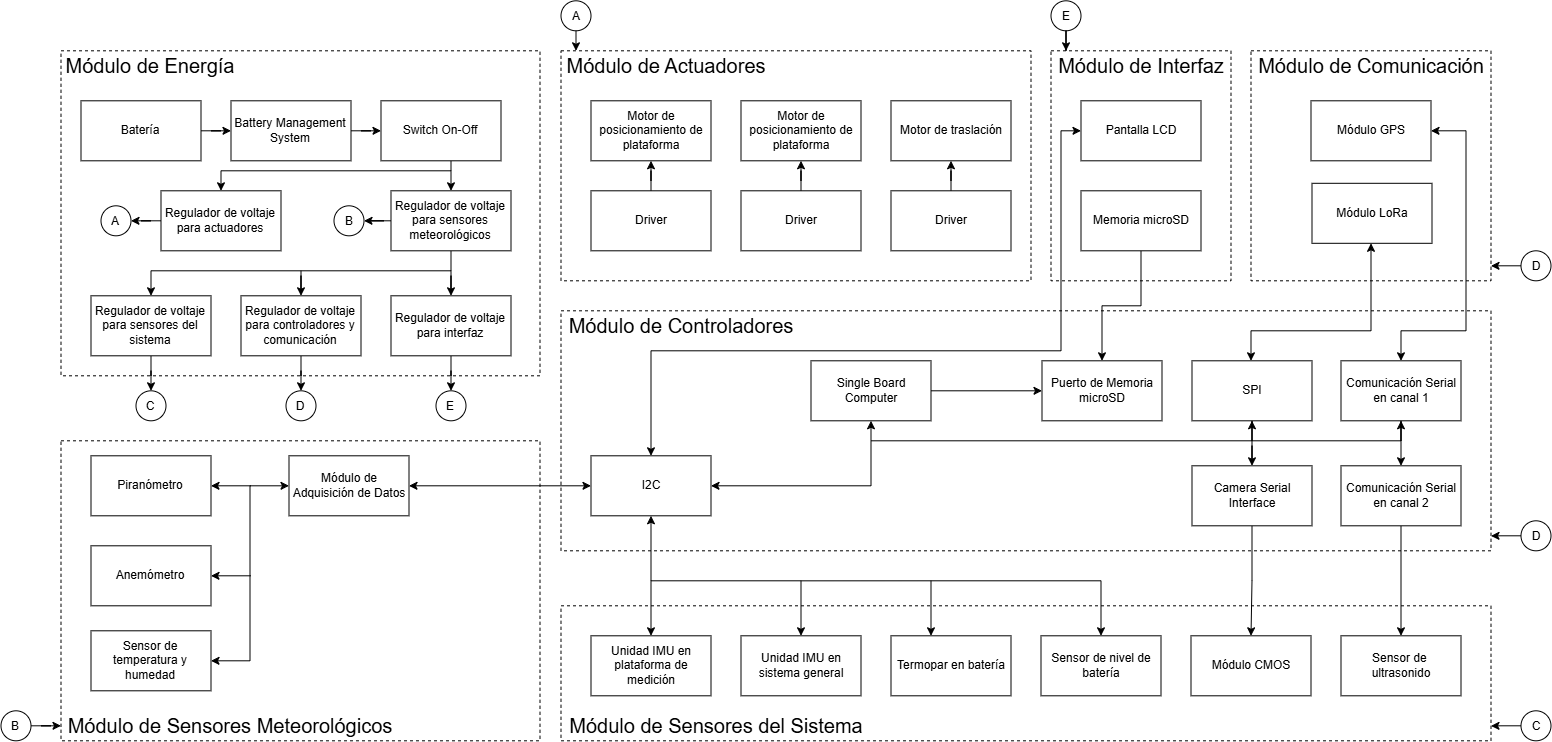
\includegraphics[width=\textwidth]{Recursos/Imagenes/ImagenesDisenoOptimo/DiagramaBloquesTFC1_v2.png} \par\medskip
	
	\raggedright
	\footnotesize \textit{Nota.} Elaboración propia.
	\label{fig:DiagramaBloques}
\end{figure}


\subsection{Selección de Materiales}

La operación continua en parques solares expone al vehículo a un rango de $10\text{ }^\circ\text{C}$ a $45\text{ }^\circ\text{C}$, alta radiación ultravioleta (UV), polvo en suspensión e impactos dinámicos de suelo irregular.

La restricción técnica principal impone una masa total inferior a $20\text{ kg}$ para garantizar la operabilidad ergonómica por parte de los supervisores de Operation \& Maintenance (O\&M), obligando a priorizar materiales con una elevada rigidez específica y una alta relación resistencia-peso. Adicionalmente, el diseño debe garantizar un grado de protección ambiental IP64 y resistencia al impacto IK08, aislando térmicamente la instrumentación meteorológica según las exigencias de la norma IEC 61724-1.

Para este análisis, los componentes del robot se dividen en tres grupos funcionales:
\begin{itemize}
    \item Estructura portante interna
    \item Carcasa exterior
    \item Mecanismos articulados y soportes de instrumentación
\end{itemize}

\subsubsection*{Estructura portante interna}

La estructura interna distribuye las cargas estáticas y dinámicas protegiendo a la electrónica y los mecanismos internos. Para esta estructura se evaluaron aleaciones ligeras frente a perfiles de acero comercial.

Como se resume en la Tabla \ref{tab:estructura_interna}, se seleccionaron los perfiles modulares de Aluminio Anodizado V-Slot. Esta aleación ofrece una densidad reducida de $2.70\text{ g/cm}^3$ y un módulo de elasticidad de $69\text{ GPa}$, logrando una rigidez flexional adecuada con un peso estructural moderado. El ranurado continuo del sistema V-Slot permite el ensamblaje y ajuste modular de los soportes internos mediante tornillería sin requerir procesos de soldadura, lo cual facilita las labores de mantenimiento preventivo y correctivo en campo.

\begin{center}
    \footnotesize
    \begin{xltabular}{\textwidth}{|p{2.8cm}|>{\centering\arraybackslash}X|>{\centering\arraybackslash}X|>{\centering\arraybackslash}X|>{\centering\arraybackslash}X|>{\centering\arraybackslash}p{3.5cm}|>{\centering\arraybackslash}X|}
        \caption{Opciones de Materiales para la Estructura Portante Interna (Bastidor)}
        \label{tab:estructura_interna} \\
        \hline
        \rowcolor[HTML]{D9E1F2} 
        \textbf{Material / Aleación} & \textbf{Densidad $\rho$ ($\text{g/cm}^3$)} & \textbf{Módulo Elástico $E$ ($\text{GPa}$)} & \textbf{Resistencia Última $\sigma_u$ ($\text{MPa}$)} & \textbf{Límite Elástico $\sigma_y$ ($\text{MPa}$)} & \textbf{Características de Ensamblaje / Maquinabilidad} & \textbf{Selección} \\ \hline
        \endfirsthead
        
        \multicolumn{7}{c}%
        {{\bfseries \tablename\ \thetable{} -- Continuación de la página anterior}} \\
        \hline
        \rowcolor[HTML]{D9E1F2} 
        \textbf{Material / Aleación} & \textbf{Densidad $\rho$ ($\text{g/cm}^3$)} & \textbf{Módulo Elástico $E$ ($\text{GPa}$)} & \textbf{Resistencia Última $\sigma_u$ ($\text{MPa}$)} & \textbf{Límite Elástico $\sigma_y$ ($\text{MPa}$)} & \textbf{Características de Ensamblaje / Maquinabilidad} & \textbf{Selección} \\ \hline
        \endhead
        
        \hline
        \endfoot
        
        \hline
        \endlastfoot
        
        Aluminio 6063-T5 (Perfil V-Slot 2020) & $2.70$ & $69.0$ & $205$ & $145$ & Modular por ranura T-Nut, sin soldadura, alta rigidez específica. & Seleccionado \\ \hline
        Aluminio 6061-T6 (Perfil Estructural) & $2.70$ & $68.9$ & $310$ & $276$ & Maquinabilidad excelente, requiere mecanizado de uniones roscadas. & Alternativa \\ \hline
        Acero Estructural A36 (Perfil Comercial) & $7.85$ & $200.0$ & $400$ & $250$ & Alta resistencia, pero penaliza críticamente la masa total ($>20\text{ kg}$). & Descartado \\ \hline
        Acero Inoxidable AISI 304 & $8.00$ & $193.0$ & $515$ & $205$ & Excelente resistencia a la corrosión, masa excesiva para UGV. & Descartado \\ \hline
    \end{xltabular}
\end{center}

\subsubsection*{Carcasa exterior}

La carcasa exterior actúa como un escudo estático que protege la electrónica central, los reguladores de voltaje y las baterías contra la acumulación de radiación solar, el ingreso de polvo y posibles impactos dinámicos durante la traslación. Se analizaron placas metálicas ligeras frente a materiales compuestos como la fibra de vidrio epóxica y láminas de acero.

Como se observa en la Tabla \ref{tab:carcasa_exterior}, se eligió la placa de Aluminio 6061-T6 de $1.5\text{ mm}$ a $2.0\text{ mm}$ de espesor. Esta aleación presenta una resistencia última a la tracción de $310\text{ MPa}$ y garantiza el cumplimiento del grado de impacto IK08 (energía de impacto de $5\text{ J}$) sin riesgo de fractura frágil. Además, su elevada conductividad térmica permite transferir por conducción el calor disipado por los drivers de tracción y la SBC hacia el exterior, evitando el sobrecalentamiento interno en entornos con temperaturas ambiente de hasta $45\text{ }^\circ\text{C}$.

\begin{center}
    \footnotesize
    \begin{xltabular}{\textwidth}{|p{2.8cm}|>{\centering\arraybackslash}X|>{\centering\arraybackslash}X|>{\centering\arraybackslash}X|>{\centering\arraybackslash}p{3.2cm}|>{\centering\arraybackslash}p{2.5cm}|>{\centering\arraybackslash}X|}
        \caption{Opciones de Materiales para la Carcasa Protectora Exterior}
        \label{tab:carcasa_exterior} \\
        \hline
        \rowcolor[HTML]{D9E1F2} 
        \textbf{Material / Configuración} & \textbf{Densidad $\rho$ ($\text{g/cm}^3$)} & \textbf{Resistencia Tracción $\sigma_u$ ($\text{MPa}$)} & \textbf{Conductividad Térmica $k$ ($\text{W/m}\cdot\text{K}$)} & \textbf{Resistencia a Impacto / Intemperie} & \textbf{Impacto en la Masa Total de Carcasa} & \textbf{Selección} \\ \hline
        \endfirsthead
        
        \multicolumn{7}{c}%
        {{\bfseries \tablename\ \thetable{} Continuación de tabla anterior}} \\
        \hline
        \rowcolor[HTML]{D9E1F2} 
        \textbf{Material / Configuración} & \textbf{Densidad $\rho$ ($\text{g/cm}^3$)} & \textbf{Resistencia Tracción $\sigma_u$ ($\text{MPa}$)} & \textbf{Conductividad Térmica $k$ ($\text{W/m}\cdot\text{K}$)} & \textbf{Resistencia a Impacto / Intemperie} & \textbf{Impacto en la Masa Total de Carcasa} & \textbf{Selección} \\ \hline
        \endhead
        
        \hline
        \endfoot
        
        \hline
        \endlastfoot
        
        Placa Aluminio 6061-T6 ($1.5\text{ mm}$) & $2.70$ & $310$ & $167.0$ & Cumple grado IK08 e IP44, alta disipación térmica. & LIGERO ($<4.5\text{ kg}$) & Seleccionado \\ \hline
        Fibra de Vidrio Epóxica (Compuesto) & $1.80$ & $220$ & $0.3$ & Aislante térmico, retiene calor interno perjudicial. & MUY LIGERO ($<3.2\text{ kg}$) & Descartado \\ \hline
        Chapa de Acero Inoxidable AISI 304 & $8.00$ & $515$ & $16.2$ & Máxima protección mecánica, nula disipación térmica. & PESADO ($>12.0\text{ kg}$) & Descartado \\ \hline
        Placa de Polímero ABS ($3.0\text{ mm}$) & $1.05$ & $45$ & $0.17$ & Degrada bajo radiación UV severa, IK08 insuficiente. & LIGERO ($<2.5\text{ kg}$) & Descartado \\ \hline
    \end{xltabular}
\end{center}

\subsubsection*{C. Mecanismos Articulados, Soportes de Instrumentación y Sellos}

Los subsistemas mecánicos activos y la suite de sensores imponen requerimientos diferenciados de límite elástico, durabilidad a la fricción y aislamiento térmico:

\begin{itemize}
    \item \textbf{Eslabones del Elevador de Tijera:} Para los brazos del pantógrafo que elevan la plataforma de medición a $h \ge 1300\text{ mm}$, se seleccionó Aluminio 7075-T6. Su elevado límite elástico soporta las cargas de flexión y fatiga mecánica inducidas por las ráfagas de viento sobre la estructura extendida.
    \item \textbf{Ejes, Husillos y Goniómetro:} Para el husillo roscado de la tijera y el par tornillo sin-fin/corona del mecanismo goniométrico (cabeceo/pitch), se empleó Acero Inoxidable AISI 304. Su bajo coeficiente de fricción reduce el desgaste mecánico y aprovecha la propiedad de autobloqueo para sostener la inclinación en el plano Tilt sin consumo eléctrico continuo del servomotor.
    \item \textbf{Soportes de Instrumentación:} Requerimiento crítico de la norma IEC 61724-1 (Clase A): Los anclajes del sensor de temperatura RTD PT100 y del anemómetro deben estar aislados térmicamente de la carcasa metálica del robot. Se seleccionó el polímero técnico PETG por su baja conductividad térmica e inalterabilidad dimensional ante radiación UV, actuando como barrera aislante para evitar transferir el calor conducido por la estructura hacia las lecturas climáticas.
\end{itemize}

\begin{center}
    \footnotesize
    \begin{xltabular}{\textwidth}{|p{3.2cm}|p{3.2cm}|p{3.2cm}|>{\centering\arraybackslash}X|}
        \caption{Selección de Materiales para Mecanismos y Soportes de Instrumentación}
        \label{tab:mecanismos_sellos} \\
        \hline
        \rowcolor[HTML]{D9E1F2} 
        \textbf{Componente / Subsistema} & \textbf{Material Seleccionado} & \textbf{Propiedad Crítica Evaluada} & \textbf{Función y Justificación Técnica / Normativa} \\ \hline
        \endfirsthead
        
        \multicolumn{4}{c}%
        {{\bfseries \tablename\ \thetable{} -- Continuación de la página anterior}} \\
        \hline
        \rowcolor[HTML]{D9E1F2} 
        \textbf{Componente / Subsistema} & \textbf{Material Seleccionado} & \textbf{Propiedad Crítica Evaluada} & \textbf{Función y Justificación Técnica / Normativa} \\ \hline
        \endhead
        
        \hline
        \endfoot
        
        \hline
        \endlastfoot
        
        Eslabones de Elevador de Tijera & Aluminio 7075-T6 & $\sigma_y = 503\text{ MPa}$, alta resistencia a fatiga & Evita deformaciones plásticas ante ráfagas de viento a $1300\text{ mm}$ de altura. \\ \hline
        Ejes y Husillo del Goniómetro & Acero Inoxidable AISI 304 & Alta resistencia al desgaste, anticorrosivo & Retención estática por autobloqueo mecánico en plano Tilt sin gasto de energía. \\ \hline
        Soportes de PT100 y Anemómetro & Polímero PETG & Conductividad térmica $k < 0.25\text{ W/m}\cdot\text{K}$ & Aislamiento térmico: Previene puentes térmicos desde el chasis metálico. \\ \hline
        Empaquetaduras y Pasacables & Caucho EPDM Industrial & Resistencia a radiación UV y rango de $-40\text{ }^\circ\text{C}$ a $120\text{ }^\circ\text{C}$ & Mantiene el sellado hermético IP44 contra el ingreso de polvo desértico y agua. \\ \hline
    \end{xltabular}
\end{center}

\subsubsection{Lazo de control del movimiento del robot}

El desplazamiento autónomo del vehículo se rige mediante un lazo de control cerrado en cascada que integra el seguimiento espacial y la regulación de velocidad. Como se observa en la Figura \ref{fig:LazoControl}, la referencia del sistema se calcula dinámicamente comparando la ruta predefinida con las coordenadas espaciales retroalimentadas por la antena GPS de parche cerámico y la orientación provista por la unidad IMU. Esta fusión de datos alimenta al algoritmo geométrico Pure Pursuit, el cual calcula el error de desvío lateral para definir el ángulo de corrección requerido.

De forma paralela, la retroalimentación de los encoders rotativos determina el error respecto a la velocidad nominal operativa de 1 m/s. El controlador central, mediante un algoritmo PID, amalgama ambos errores para generar y distribuir las señales de Modulación por Ancho de Pulsos hacia los actuadores. Al tratarse de un chasis de tracción diferencial, el PID varía la potencia entre los flancos izquierdo y derecho para corregir el rumbo y mantener al robot sobre la trayectoria ideal sin interrumpir su avance.

\begin{figure}[H]
	\captionsetup{justification=raggedright, singlelinecheck=false, labelsep=none}
	
	\caption[Lazo de control del movimiento de traslación del robot.]{} 
	
	\textit{Lazo de control del movimiento de traslación del robot.} \par\medskip
	
	\centering
	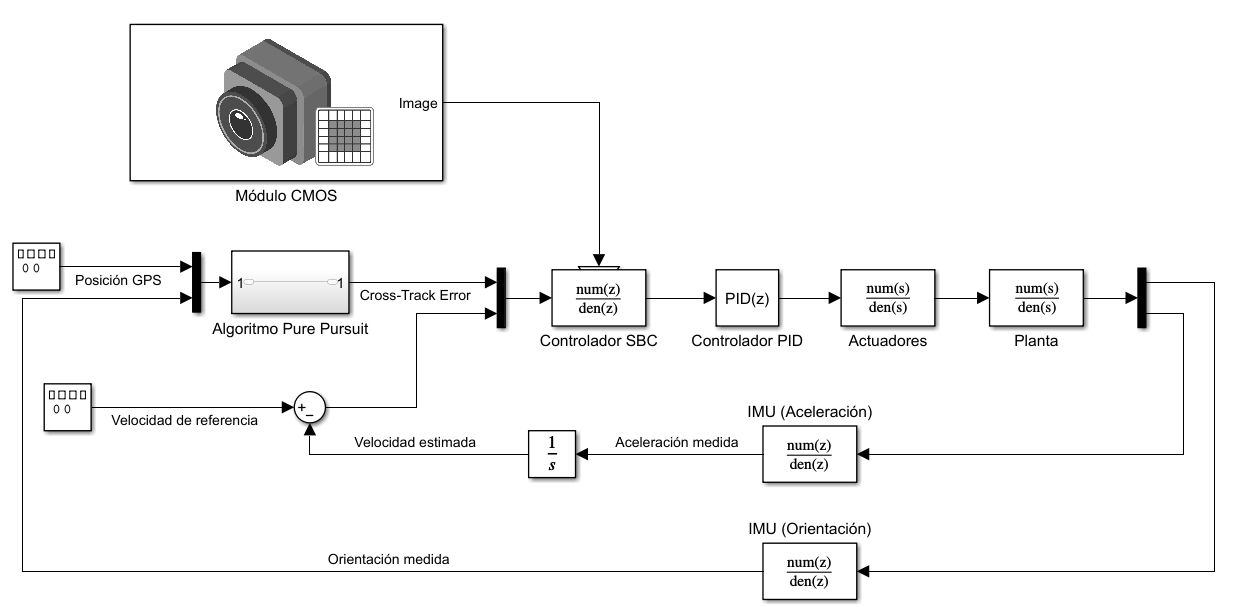
\includegraphics[width=\textwidth]{Recursos/Imagenes/ImagenesDisenoOptimo/LazoControlNavegación.png} \par\medskip
	
	\raggedright
	\footnotesize \textit{Nota.} Elaboración propia.
	\label{fig:LazoControl}
\end{figure}

Por otro lado, el control de los subsistemas de altura y orientación se rige mediante un lazo de control cerrado simple que integran los sensores IMU y de ultrasonido con referencias estáticas. Como se observa en la Figura \ref{fig:LazosControl}.

\begin{figure}[H]

	\captionsetup{justification=raggedright, singlelinecheck=false, labelsep=none}
	
	\caption[Lazo de control para el ajuste altura y orientación del sensor de irradiancia.]{} 
	
	\textit{Lazo de control para el ajuste altura (izquierda) y orientación (derecha) del sensor de irradiancia.} \par\medskip
	
	\begin{minipage}{0.5\textwidth}
		\centering
		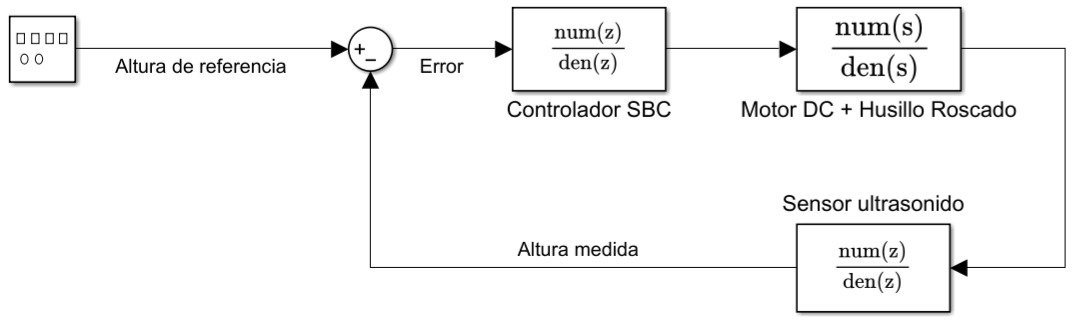
\includegraphics[width=\linewidth]{Recursos/Imagenes/ImagenesDisenoOptimo/LazoControlAltura.jpg}
	\end{minipage}\hfill
	\begin{minipage}{0.5\textwidth}
		\centering
		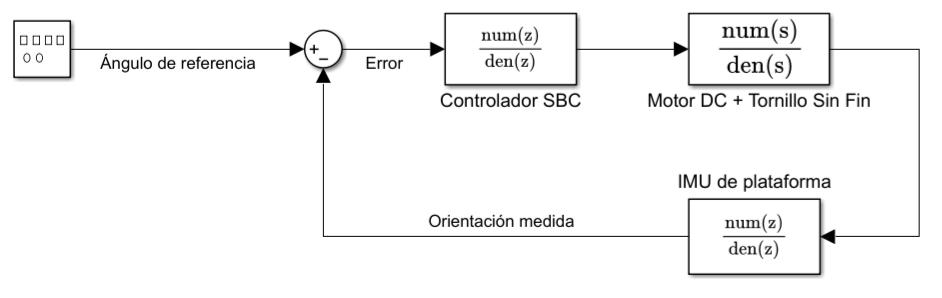
\includegraphics[width=\linewidth]{Recursos/Imagenes/ImagenesDisenoOptimo/LazoControlAngulo.png}
	\end{minipage}
	\par\medskip
	
	\raggedright
	\footnotesize \textit{Nota.} Elaboración propia..
	\label{fig:LazosControl}
\end{figure}

\subsubsection{Topología de red}

La arquitectura de comunicaciones, vista en la Figura \ref{fig:TopologiaRed}, del sistema emplea una topología punto a punto fundamentada en el protocolo de radiofrecuencia LoRa. En este esquema, el robot de inspección actúa como un nodo terminal móvil equipado con un módulo transceptor LoRa que concentra los datos meteorológicos procesados.

La capa de red establece un enlace bidireccional de baja potencia y largo alcance con la estación base o Gateway ubicada en las instalaciones del parque fotovoltaico, garantizando una cobertura efectiva superior a los 200 metros. El enlace de subida se encarga de transmitir los paquetes de telemetría y alertas de obstáculos hacia el servidor central para su visualización y almacenamiento, mientras que el enlace de bajada permite que el dispositivo escuche continuamente comandos del exterior, posibilitando la recepción de instrucciones críticas como el telecomando de parada remota emitido por el operario.

\begin{figure}[H]
	\captionsetup{justification=raggedright, singlelinecheck=false, labelsep=none}
	
	\caption[Topología de red con los robots como nodos.]{} 
	
	\textit{Topología de red con los robots como nodos.} \par\medskip
	
	\centering
	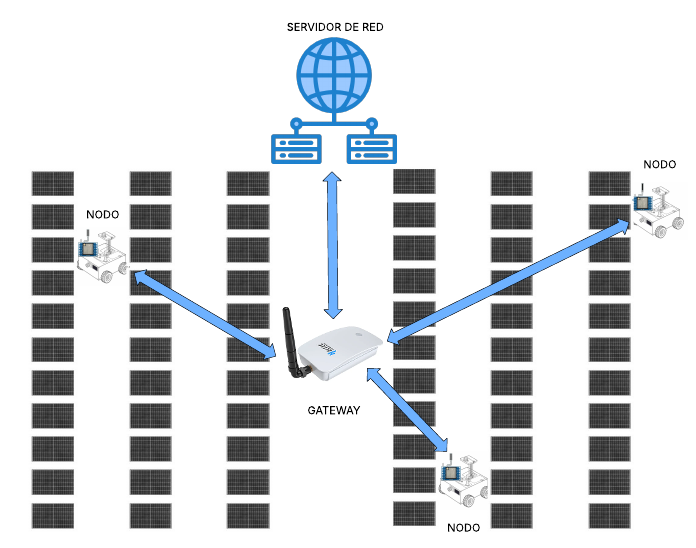
\includegraphics[width=\textwidth]{Recursos/Imagenes/ImagenesDisenoOptimo/TopologiaRedTFC1.png} \par\medskip
	
	\raggedright
	\footnotesize \textit{Nota.} Elaboración propia.
	\label{fig:TopologiaRed}
\end{figure}

\subsubsection{Diagrama de flujo general} 

En la Figura \ref{fig:DiagramaFlujoGeneral}, se detalla la secuencia lógica de arranque y la arquitectura multitarea que gobierna la computadora principal del robot. El proceso inicia con la energización del hardware, donde el sistema operativo inicializa los buses de comunicación y declara una variable global de estado o Flag de Alerta en valor nulo. Posteriormente, el equipo entra en un estado de espera hasta recibir el comando inalámbrico de inicio por parte del operario.

Una vez activado, el software ejecuta una bifurcación propia de arquitecturas orientadas a eventos, dividiendo el procesamiento en hilos paralelos que operan de forma concurrente: un hilo de navegación, un hilo de telemetría y un hilo supervisor de seguridad. En lugar de que cada subproceso gestione sus propias condiciones de parada, los hilos paralelos operan exclusivamente como publicadores de estado. Simultáneamente, el hilo supervisor evalúa la Flag de Alerta de forma continua; si detecta un cambio de estado a valor activo, el supervisor ejecuta una interrupción de máxima prioridad que anula la tracción y transita al sistema hacia un modo seguro.

\begin{figure}[H]
	\captionsetup{justification=raggedright, singlelinecheck=false, labelsep=none}
	
	\caption[Diagrama de flujo de proceso general.]{} 
	
	\textit{Diagrama de flujo de proceso general.} \par\medskip
	
	\centering
	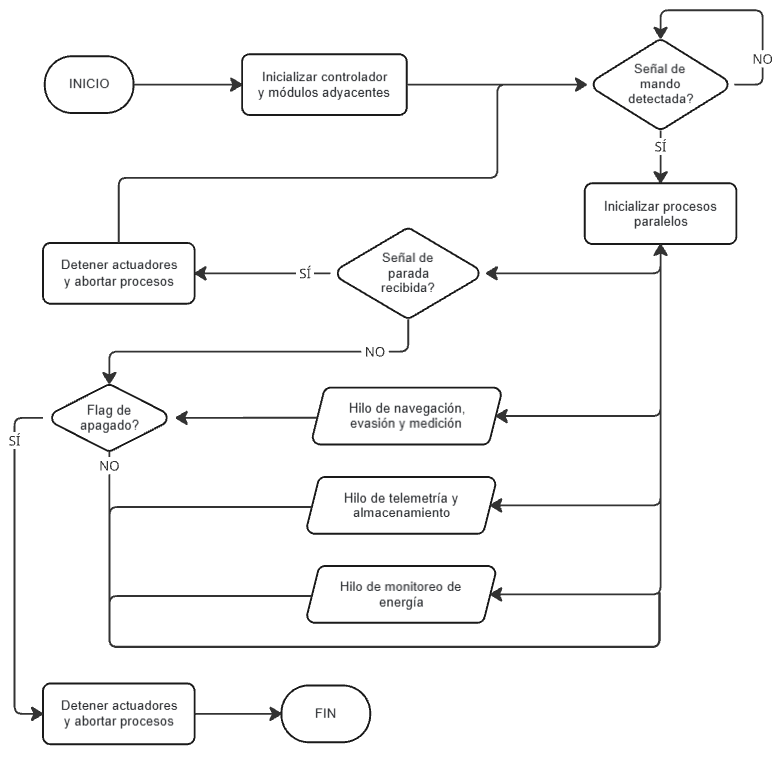
\includegraphics[width=\textwidth]{Recursos/Imagenes/ImagenesDisenoOptimo/FlujoPrincipal.png} \par\medskip
	
	\raggedright
	\footnotesize \textit{Nota.} Elaboración propia.
	\label{fig:DiagramaFlujoGeneral}
\end{figure}

\subsubsection{Variables de control}
\begin{center}
    \footnotesize
    \begin{xltabular}{\textwidth}{|p{4.0cm}|p{3.5cm}|>{\centering\arraybackslash}p{2.2cm}|>{\centering\arraybackslash}X|}
        \caption{EDT 2.2.2 --- Variables por Monitorear / Controlar}
        \label{tab:variables_monitoreo_control} \\
        \hline
        \rowcolor[HTML]{D9E1F2} 
        \textbf{Variable} & \textbf{Tipo de Señal} & \textbf{Monitorear / Controlar} & \textbf{Acción / Descripción} \\ \hline
        \endfirsthead
        
        \multicolumn{4}{c}%
        {{\bfseries \tablename\ \thetable{} -- Continuación de la página anterior}} \\
        \hline
        \rowcolor[HTML]{D9E1F2} 
        \textbf{Variable} & \textbf{Tipo de Señal} & \textbf{Monitorear / Controlar} & \textbf{Acción / Descripción} \\ \hline
        \endhead
        
        \hline
        \endfoot
        
        \hline
        \endlastfoot
        
        Irradiancia global TILT & Analógica & Monitorear & Registro de lectura en plano de paneles fotovoltaicos. \\ \hline
        Variables climáticas secundarias  & Analógica & Monitorear & Muestreo cada 5 s. \\ \hline
        Velocidad diferencial & Salida PWM & Controlar & Regulación de la velocidad de avance a $1\text{ m/s}$ nominal. \\ \hline
        Posición vertical de tijera & Salida PWM / Digital & Controlar & Despliegue de elevación a la altura $h \ge 1300\text{ mm}$ del suelo. \\ \hline
        Ángulo goniométrico& Salida PWM / Digital & Controlar & Alineación angular del piranómetro en el plano de inclinación de los paneles. \\ \hline
        Coordenadas GPS y Vectores IMU  & UART / I2C / SPI & Monitorear & Fusión de sensores para estimación de postura y navegación con Pure Pursuit. \\ \hline
        Estado de Batería Li-Ion & I2C / ADC & Monitorear & Monitoreo de porcentaje de carga mediante contador de Culombios del BMS. \\ \hline
    \end{xltabular}
\end{center}

\subsubsection{Implementación de software}
\subsubsection{Selección del controlador principal}

\subsection{Diseño de interfaz de usuario}
\subsubsection{Pantalla de bienvenida y autenticación del operador}
\subsubsection{Panel principal}
\subsubsection{Menú de usuario y carga de rutas de inspección}
\subsubsection{Pantalla de mantenimiento}
\subsubsection{Sistema de alertas}
\subsubsection{Interfaz física de usuario}

\subsection{Diseño del subsistema estructural}
\subsubsection{Diseño de estructura externa}
\subsubsection{Diseño de soporte funcional}

\subsection{Diseño del subsistema de elevación por pantógrafo}

\subsection{Diseño del subsistema de mecanismo goniométrico}

\subsection{Diseño del subsistema de tracción diferencial}

\subsection{Diseño del subsistema de comunicaciones y telemetría}

\subsection{Diseño del subsistema de navegación autónoma}

\subsection{Selección de sensores}

\subsection{Selección de actuadores}

\section{Modelado 3D y planos de fabricación del sistema}

\section{Diseño de circuito impreso y esquemáticos de conexión}

\section{Simulación y validación digital}

\section{Presupuesto detallado, lista de materiales y estimación de costos de capital}